\section{非齐次线性方程组}

\subsection{方程组与行列式}

\begin{example}
    已知线性方程组 $\left\{\begin{matrix}
            ax_1 & + &      &   & x_3  & = & 1 \\
            x_1  & + & ax_2 & + & x_3  & = & 0 \\
            x_1  & + & 2x_2 & + & ax_3 & = & 0 \\
            ax_1 & + & bx_2 &   &      & = & 2
        \end{matrix}\right.$ 有解, 其中 $a,b$ 为常数, 若 $\mqty|a&0&1\\1&a&1\\1&2&a|=4$, 求 $\mqty|1&a&1\\1&2&a\\a&b&0|.$
\end{example}
\begin{solution}
    设 $\vb*{x}$ 的系数矩阵为 $\vb*{A}$, $(1,0,0,2)^\top=\vb*{b}$, 因为方程组有解, 则 $\rank(\vb*{A},\vb*{b})=\rank(\vb*{A})$, 由于 $\mqty|a&0&1\\1&a&1\\1&2&a|=4\neq0$, 所以 $\rank\vb*{A}\geqslant 3$,
    又因为 $\vb*{A}_{4\times3}$, 所以 $\rank\vb*{A}\leqslant 3$, 于是 $$\rank\vb*{A}=3\Rightarrow \rank(\vb*{A},\vb*{b})=3\Rightarrow\det(\vb*{A},\vb*{b})=0$$
    对行列式 $\det(\vb*{A},\vb*{b})$ 按最后一列展开, 得
    $$\det(\vb*{A},\vb*{b})=-\mqty|1&a&1\\1&2&a\\a&b&0|+2\mqty|a&0&1\\1&a&1\\1&2&a|\Rightarrow\mqty|1&a&1\\1&2&a\\a&b&0|=8. $$
\end{solution}

\subsection{Cramer 法则的应用}

\begin{theorem}[Cramer 法则]\index{Cramer 法则}
    如果数域 $ K $ 上的含有 $ n $ 个末知量 $ n $ 个方程的线性方程组
    $$\begin{cases}
            a_{11} x_{1}+a_{12} x_{2}+\cdots+a_{1 n} x_{n}=b_{1}                  \\
            a_{21} x_{1}+a_{22} x_{2}+\cdots+a_{2 n} x_{n}=b_{2}                  \\
            \cdots \cdots \cdots \cdots \cdots \cdots \cdots \cdots \cdots \cdots \\
            a_{n 1} x_{1}+a_{n 2} x_{2}+\cdots+a_{n n} x_{n}=b_{n}
        \end{cases}$$
    的系数行列式 $ D \neq 0$, 那么此方程组有唯一解 $ \left(\dfrac{D_{1}}{D}, \dfrac{D_{2}}{D}, \cdots, \dfrac{D_{n}}{D}\right)$,
    其中 $ D_{j} $ 是把 $ D $ 中第 $ j $ 列的元素换成方程组的常数项 $ b_{1}, b_{2}, \cdots, b_{n} $ 而成的行列式 $ (j=1,2, \cdots, n)$, 即
    $$\mqty|a_{11}  & \cdots & a_{1, j-1} & b_{1}  & a_{1, j+1} & \cdots & a_{1 n} \\
        a_{21}  & \cdots & a_{2, j-1} & b_{2}  & a_{2, j+1} & \cdots & a_{2 n} \\
        \vdots  &        & \vdots     & \vdots & \vdots     &        & \vdots  \\
        a_{n 1} & \cdots & a_{n, j-1} & b_{n}  & a_{n, j+1} & \cdots & a_{n n}|$$
    特别地, 当 $ b_{i}=0(i=1,2, \cdots, n) $ 时, 如果系数行列式 $ D \neq 0 $, 那么方程组只有零解;
    反之, 如果方程组有非零解,那么必有 $ D=0 .$
\end{theorem}

\begin{example}[2005 华中科技大学]
    解线性方程组 $\begin{cases}
            x_1+ax_2+a^2x_3=a^3 \\
            x_1+bx_2+b^2x_3=b^3 \\
            x_1+cx_2+c^2x_3=c^3 \\
        \end{cases}$
    其中 $a,b,c$ 是互不相等的常数.
\end{example}
\begin{solution}
    利用 Cramer 法则求解, 因为系数行列式 $$D=\mqty|1&a&a^2\\1&b&b^2\\1&c&c^2|=(c-b)(c-a)(b-a)\neq0$$
    所以方程组有唯一解, 又因为
    $$D_1=\mqty|a^3&a&a^2\\b^3&b&b^2\\b^3&b&b^2|=abcD,~D_2=\mqty|1&a^3&a^2\\1&b^3&b^2\\1&c^3&c^2|=-(ab+ac+bc)D,~D_3=\mqty|1&a&a^3\\1&b&b^3\\1&c&c^3|=(a+b+c)D$$
    因此 $x_1=\dfrac{D_1}{D}=abc,~x_2=\dfrac{D_2}{D}=-ab-ac-bc,~x_3=\dfrac{D_3}{D}=a+b+c.$
\end{solution}

\subsection{线性相关与线性无关}

\subsubsection{线性无关}

\begin{example}[2009 数一]
    设 $\vb*{A}=\mqty(1&-1&-1\\-1&1&1\\0&-4&-2),~\vb*{\xi}_1=\mqty(-1\\1\\-2)$,
    \begin{enumerate}[label=(\arabic{*})]
        \item 求满足 $\vb*{A\xi}_2=\vb*{\xi}_1,~\vb*{A}^2\vb*{\xi}_3=\vb*{\xi}_1$ 的所有向量 $\vb*{\xi}_2,~\vb*{\xi}_3$;
        \item 对 (1) 中的任意向量 $\vb*{\xi}_2,~\vb*{\xi}_3$, 证明: $\vb*{\xi}_1,\vb*{\xi}_2,\vb*{\xi}_3$ 线性无关.
    \end{enumerate}
\end{example}
\begin{solution}
    \begin{enumerate}[label=(\arabic{*})]
        \item 对矩阵 $(\vb*{A},\vb*{\xi}_1)$ 施行初等行变换, 得
              $$(\vb*{A},\vb*{\xi}_1)=\begin{pNiceArray}{ccc:c}
                      1  & -1 & -1 & -1 \\
                      -1 & 1  & 1  & 1  \\
                      0  & -4 & -2 & -2
                  \end{pNiceArray}\to\begin{pNiceArray}{ccc:c}
                      1 & 0 & -\dfrac{1}{2} & -\dfrac{1}{2} \\[6pt]
                      0 & 1 & \dfrac{1}{2}  & \dfrac{1}{2}  \\[6pt]
                      0 & 0 & 0             & 0
                  \end{pNiceArray}$$
              由此可解得 $\vb*{\xi}_2=\mqty(-\dfrac{1}{2}+\dfrac{k}{2},\dfrac{1}{2}-\dfrac{k}{2},k)^\top$, 其中 $k$ 为任意常数,
              再对矩阵 $(\vb*{A}^2,\vb*{\xi}_1)$ 施行初等行变换, 得
              $$(\vb*{A}^2,\vb*{\xi}_1)=\begin{pNiceArray}{ccc:c}
                      2  & 2  & 0 & -1 \\
                      -2 & -2 & 0 & 1  \\
                      4  & 4  & 0 & -2
                  \end{pNiceArray}\to\begin{pNiceArray}{ccc:c}
                      1 & 1 & 0 & -\dfrac{1}{2} \\[6pt]
                      0 & 0 & 0 & 0             \\
                      0 & 0 & 0 & 0
                  \end{pNiceArray}$$
              故可解得 $\vb*{\xi}_3=\mqty(-\dfrac{1}{2}-a,b)^\top$, 其中 $a,b$ 为任意常数.
        \item 由 (1) 的结果, 有
              \begin{flalign*}
                  \qty|\vb*{\xi}_1,\vb*{\xi}_2,\vb*{\xi}_3|=\mqty|-1 & \dfrac{k-1}{2} & -\dfrac{1}{2}-a \\[6pt]1&\dfrac{1-k}{2}&a\\[6pt]-2&k&b|\xlongequal{r_1+r_2}\mqty|0&0&-\dfrac{1}{2}\\[6pt]1&\dfrac{1-k}{2}&a\\[6pt]-2&k&b|=-\dfrac{1}{2}\neq0
              \end{flalign*}
              所以 $\vb*{\xi}_1,\vb*{\xi}_2,\vb*{\xi}_3$ 线性无关.
    \end{enumerate}
\end{solution}

\subsection{非齐次线性方程组解的讨论}

\begin{theorem}[非齐次线性方程组有解的条件]
    $n$ 元非齐次线性方程组 $\vb*{Ax}=\vb*{b}$ 解的情况:\index{非齐次线性方程组有解的条件}
    \begin{enumerate}[label=(\arabic{*})]
        \item 方程组 $\vb*{Ax}=\vb*{b}$ 有唯一解 $\Leftrightarrow \rank\vb*{A}=\rank\bar{\vb*{A}}=n$;
        \item 方程组 $\vb*{Ax}=\vb*{b}$ 有无穷多解 $\Leftrightarrow \rank\vb*{A}=\rank\bar{\vb*{A}}<n$;
        \item 方程组 $\vb*{Ax}=\vb*{b}$ 无解 $\Leftrightarrow \rank\vb*{A}\neq\rank\bar{\vb*{A}}$.
    \end{enumerate}
\end{theorem}

\subsubsection{方程组无解的充要条件}

\begin{example}[2000 数一]
    已知方程组 $\begin{pmatrix} 1 & 2 & 1 \\ 2 & 3 & a+2 \\ 1 & a & -2 \\\end{pmatrix}\mqty( x_1 \\ x_2  \\ x_n )=\mqty( 1 \\ 3  \\ 0 )$ 无解, 求 $a$.
\end{example}
\begin{solution}
    方程组无解的充要条件是 $\rank\vb*{A}\neq\rank\vb*{\bar{A}}$, 故应对增广矩阵作初等行变换, 由 
    $$
    \begin{pNiceArray}{ccc:c}
        1 & 2 & 1 & 1 \\ 2 & 3 & a+2 & 3 \\ 1 & a & -2 & 0
    \end{pNiceArray}\xrightarrow[r_3-r_1]{r_2-2r_1}\begin{pNiceArray}{ccc:c}
        1 & 2 & 1 & 1 \\ 0 & -1 & a & 1 \\ 0 & a-2 & -3 & -1
    \end{pNiceArray}\xrightarrow{r_3+(a-2)\times r_2}\begin{pNiceArray}{ccc:c}
        1 & 2 & 1 & 1 \\ 0 & -1 & a & 1 \\ 0 & 0 & a^2-2a-3 & a-3
    \end{pNiceArray}
    $$
    可知, 若 $a=-1$, 则 $\vb*{\bar{A}}\to\begin{pNiceArray}{ccc:c}
        1 & 2 & 1 & 1 \\ 0 & -1 & -1 & 1 \\ 0 & 0 & 0 & -4
    \end{pNiceArray}$, 于是 $\rank\vb*{A}=2, \rank\vb*{\bar{A}}=3$, 从而方程组无解, 因此 $a=-1.$
\end{solution}

% \subsubsection{无穷多解}

% \begin{example}
%     设方程组 $\begin{pmatrix} a & 1 & 1 \\ 1 & a & 1 \\ 1 & 1 & a \\\end{pmatrix}\mqty( x_1 \\ x_2 \\ x_n )=\mqty(1\\1\\-2)$ 有无穷多解, 求 $a$.
% \end{example}
% \begin{solution}
%     对增广矩阵 $\vb*{\bar{A}}$ 作初等行变换化为行最简单形:
    
% \end{solution}

\begin{example}[2016 南京大学]
    讨论当 $a,b$ 为何值时, 线性方程组
    $$\left\{\begin{array}{rrrrrrrrrrr}
            x_{1}   & + & x_{2}   & + & x_{3}   & + & x_{4}   & + & x_{5}   & = & 1 \\
            3 x_{1} & + & 2 x_{2} & + & x_{3}   & + & x_{4}   & - & 3x_{5}  & = & a \\
                    &   & x_{2}   & + & 2 x_{3} & + & 2 x_{4} & + & 6 x_{5} & = & 3 \\
            5 x_{1} & + & 4 x_{2} & + & 3 x_{3} & + & 3 x_{4} & - & x_{5}   & = & b
        \end{array}\right.$$
    有解? 无解? 并求出有解时的一般解.
\end{example}
\begin{solution}
    对方程组的增广矩阵施行初等行变换, 化为简化的行阶梯形矩阵:
    $$\begin{pNiceArray}{c:c}
            \vb*{A} & \vb*{B}
        \end{pNiceArray}\xrightarrow[r_1-r_3]{\substack{r_2-3r_1+r_3\\r_4-5r_1+r_3}}
        \begin{pNiceArray}{ccccc:c}
            1 & 0 & -1 & -1 & -5 & -2  \\
            0 & 1 & 2  & 2  & 6  & 3   \\
            0 & 0 & 0  & 0  & 0  & a   \\
            0 & 0 & 0  & 0  & 0  & b-2
        \end{pNiceArray}$$
    \begin{enumerate}[label=(\arabic{*})]
        \item 当 $a\neq0$ 或 $b\neq2$ 时, 方程组无解;
        \item 当 $a=0$ 且 $b=2$ 时, 方程组有解, 此时, 方程组的一般解为
              $$\vb*{x}=\mqty(-2\\3\\0\\0\\0)+k_1\mqty(1\\-2\\1\\0\\0)+k_2\mqty(1\\-2\\0\\1\\0)+k_3\mqty(5\\-6\\0\\0\\1)$$
              其中 $k_1,k_2,k_3$ 为任意常数.
    \end{enumerate}
\end{solution}

\subsubsection{方程组解的结构与通解}

\begin{example}
    已知 $\vb*{\xi}_1=(-9,1,2,11)^\top, \vb*{\xi}_2=(1,-5,13,0)^\top, \vb*{\xi}_3=(-7,-9,24,11)^\top$ 是方程组
    $$
    \begin{cases}
        a_1x_1+7x_2+a_3x_3+x_4=d_1\\ 3x_1+b_2x_2+2x_3+2x_4=d_2\\9x_1+4x_2+x_3+7x_4=2
    \end{cases}
    $$的解, 求方程组的通解.
\end{example}
\begin{solution}
    只要知道 $\rank\vb*{A}$, 算出 $n-\rank\vb*{A}$ 就知道解的结构, 因为矩阵 $\vb*{A}=\begin{pmatrix} a_1 & 7 & a_3 & 1\\ 3 & b_2 & 2 & 2\\ 9 & 4 & 1 & 7\\\end{pmatrix}$ 中有二阶子式 $\mqty|2&2\\1&7|\neq0$, 所以 $\rank\vb*{A}\geqslant 2$, 又 
    $$
    \vb*{xi}_1-\vb*{xi}_2=(-10,6,-11,11)^\top, \quad \vb*{xi}_1-\vb*{xi}_3=(-2,10,-22,0)^\top
    $$
    是齐次方程组 $\vb*{Ax}=\vb*{0}$ 的两个线性无关的解, 而有 $$4-\rank\vb*{A}\geqslant 2\Rightarrow \rank\vb*{A}\leqslant 2$$
    从而得 $\rank\vb*{A}=2$, 所以方程组的通解为 $\mqty(-9\\1\\2\\11)+k_1\mqty(-10\\6\\-11\\11)+k_2\mqty(-1\\5\\-11\\0),\forall k_1,k_2\in \mathbb{R}.$
\end{solution}

\begin{example}[2014 数一]
    设 $\vb*{A}=\mqty(1&-2&3&-4\\0&1&-1&1\\1&2&0&-3)$, $\vb*{E}$ 为 $3$ 阶矩阵,
    \begin{enumerate}[label=(\arabic{*})]
        \item 求方程组 $\vb*{Ax}=\vb*{0}$ 的一个基础解系;
        \item 求满足 $\vb*{AB}=\vb*{E}$ 的所有矩阵 $\vb*{B}$.
    \end{enumerate}
\end{example}
\begin{solution}
    \begin{enumerate}[label=(\arabic{*})]
        \item 对矩阵 $\vb*{A}$ 作初等行变换化为行最简单形, 有
        $$
        \vb*{A}=\mqty(1&-2&3&-4\\0&1&-1&1\\1&2&0&-3)\xrightarrow{r_3-r_1-4r_2}\mqty(1&-2&3&-4\\0&1&-1&1\\0&0&1&-3)\xrightarrow[r_1+2r_2-3r_3]{r_2+r_3}\mqty(1&0&0&1\\0&1&0&-2\\0&0&1&-3)
        $$
        因 $n-\rank\vb*{A}=4-3=1$, 令 $x_4=1$, 则有 $x_3=3, x_2=2, x_1=-1$, 因此基础解系为 $\vb*{\eta}=(-1,2,3,1)^\top.$
        \item $\vb*{AB}=\vb*{E}$ 中 $\vb*{B}$ 的列向量其实是三个非齐次线性方程组
        $$
        \vb*{Ax}=\mqty(1\\0\\0),\quad\vb*{Ax}=\mqty(0\\1\\0),\quad\vb*{Ax}=\mqty(0\\0\\1)
        $$
        的解, 由于这三个方程组的系数矩阵是相同的, 所以令 $\vb*{\bar{A}}=(\vb*{A},\vb*{E})$ 作初等行变换, 
        \begin{flalign*}
            \vb*{\bar{A}}=\begin{pNiceArray}{cccc:ccc}1&-2&3&-4&1&0&0\\0&1&-1&1&0&1&0\\1&2&0&-3&0&0&1\end{pNiceArray}\xrightarrow[\substack{r_2+r_3\\ r_1+2r_2-3r_3}]{r_3-r_1-4r_2}
            \begin{pNiceArray}{cccc:ccc}1&0&0&1&2&6&-1\\0&1&0&-2&-1&-3&1\\0&0&1&-3&-1&-4&1\end{pNiceArray}
        \end{flalign*}
        由此解得三个方程组的通解 
        $$
        (-2,-1,-1,0)^\top+k_1\vb*{\eta},\quad
        (6,-3,-4,0)^\top+k_2\vb*{\eta},\quad
        (-1,1,1,0)^\top+k_3\vb*{\eta}
        $$
        因此 $\vb*{B}=\mqty(2-k_1&6+2k_2&-1-k_3\\-1+2k_1&-3+2k_2&1+2k_3\\-3+3k_1&-4+3k_2&1+3k_2\\k_1&k_2&k_3),\forall k_1, k_2, k_3\in\mathbb{R}.$
    \end{enumerate}
\end{solution}

\subsection{线面关系}

\subsubsection{直线与直线之间的位置关系}

\begin{theorem}[线线关系]
    系数矩阵 $\vb*{A}=\mqty(a_1&b_1\\a_2&b_2\\a_3&b_3)$, 增广矩阵 $\bar{\vb*{A}}=\mqty(a_1&b_1&c_1\\a_2&b_2&c_2\\a_3&b_3&c_3)$, 法向量 $\vb*{n}_i=(a_i,b_i)~i=1,2,3$, 则 
    $$
    \begin{cases}
        \text{唯一解: 化简后法向量仍有 2 个, 方程变为 2 个, 如图 \ref{xxfczjiheyy}(a), } \rank\vb*{A}=\rank\bar{\vb*{A}}=2\\ 
        \text{无穷多解: }
            \text{三条直线重合, 如图 \ref{xxfczjiheyy}(b), }\rank\vb*{A}=\rank\bar{\vb*{A}}=1\\ 
        \text{无解: }\begin{cases}
            \text{化简后法向量仍有 2 个, 方程变为 3 个, 2 个交点, 如图 \ref{xxfczjiheyy}(c), }\rank\vb*{A}=2\neq\rank\bar{\vb*{A}}=3\\ 
            \text{化简后法向量仍有 2 个, 方程变为 3 个, 3 个交点, 如图 \ref{xxfczjiheyy}(d), }\rank\vb*{A}=2\neq\rank\bar{\vb*{A}}=3\\ 
            \text{两条直线重合, 法向量仍有 1 个, 方程变为 2 个, 如图 \ref{xxfczjiheyy}(e), }\rank\vb*{A}=1\neq\rank\bar{\vb*{A}}=2\\ 
            \text{三条直线互不重叠, 且相互平行, 如图 \ref{xxfczjiheyy}(f), }\rank\vb*{A}=1\neq\rank\bar{\vb*{A}}=3\\ 
        \end{cases}
    \end{cases}
    $$
\end{theorem}

\begin{figure}[H]
    \centering
    \subfigure[scale=.9][$r(\vb*{A})=r(\bar{\vb*{A}})=2$]{
        

\tikzset{every picture/.style={line width=0.75pt}} %set default line width to 0.75pt        

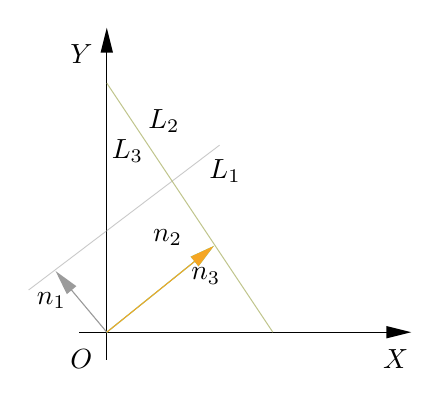
\begin{tikzpicture}[x=0.75pt,y=0.75pt,yscale=-1,xscale=1]
%uncomment if require: \path (0,310); %set diagram left start at 0, and has height of 310

%Straight Lines [id:da8559030818950601] 
\draw    (193.33,200.55) -- (193.33,173.89) -- (193.33,147.22) -- (193.33,120.55) -- (193.33,93.89) -- (193.33,67.22) -- (193.33,42.55) ;
\draw [shift={(193.33,40.55)}, rotate = 90] [fill={rgb, 255:red, 0; green, 0; blue, 0 }  ][line width=0.08]  [draw opacity=0] (12,-3) -- (0,0) -- (12,3) -- cycle    ;
%Straight Lines [id:da7578923312212116] 
\draw    (180,187.22) -- (206.67,187.22) -- (233.33,187.22) -- (260,187.22) -- (286.67,187.22) -- (313.33,187.22) -- (338,187.22) ;
\draw [shift={(340,187.22)}, rotate = 180] [fill={rgb, 255:red, 0; green, 0; blue, 0 }  ][line width=0.08]  [draw opacity=0] (12,-3) -- (0,0) -- (12,3) -- cycle    ;
%Straight Lines [id:da9090260200549443] 
\draw [color={rgb, 255:red, 155; green, 155; blue, 155 }  ,draw opacity=1 ][fill={rgb, 255:red, 155; green, 155; blue, 155 }  ,fill opacity=1 ]   (193.33,187.22) -- (169.95,159.3) ;
\draw [shift={(168.67,157.77)}, rotate = 50.05] [fill={rgb, 255:red, 155; green, 155; blue, 155 }  ,fill opacity=1 ][line width=0.08]  [draw opacity=0] (12,-3) -- (0,0) -- (12,3) -- cycle    ;
%Straight Lines [id:da5770011809774662] 
\draw [color={rgb, 255:red, 80; green, 227; blue, 194 }  ,draw opacity=1 ][fill={rgb, 255:red, 155; green, 155; blue, 155 }  ,fill opacity=1 ]   (193.33,187.22) -- (243.4,146.87) ;
\draw [shift={(244.96,145.62)}, rotate = 141.14] [fill={rgb, 255:red, 80; green, 227; blue, 194 }  ,fill opacity=1 ][line width=0.08]  [draw opacity=0] (12,-3) -- (0,0) -- (12,3) -- cycle    ;
%Straight Lines [id:da8716693688878683] 
\draw [color={rgb, 255:red, 245; green, 166; blue, 35 }  ,draw opacity=1 ][fill={rgb, 255:red, 155; green, 155; blue, 155 }  ,fill opacity=1 ]   (193.33,187.22) -- (243.4,146.87) ;
\draw [shift={(244.96,145.62)}, rotate = 141.14] [fill={rgb, 255:red, 245; green, 166; blue, 35 }  ,fill opacity=1 ][line width=0.08]  [draw opacity=0] (12,-3) -- (0,0) -- (12,3) -- cycle    ;
%Straight Lines [id:da11292330198066391] 
\draw [color={rgb, 255:red, 155; green, 155; blue, 155 }  ,draw opacity=0.35 ][fill={rgb, 255:red, 155; green, 155; blue, 155 }  ,fill opacity=1 ]   (247.67,97.1) -- (155.67,166.89) ;
%Straight Lines [id:da016532752645044724] 
\draw [color={rgb, 255:red, 80; green, 227; blue, 194 }  ,draw opacity=0.35 ][fill={rgb, 255:red, 155; green, 155; blue, 155 }  ,fill opacity=1 ]   (193.33,67.22) -- (273.33,187.22) ;
%Straight Lines [id:da18656387509211325] 
\draw [color={rgb, 255:red, 245; green, 166; blue, 35 }  ,draw opacity=0.35 ][fill={rgb, 255:red, 155; green, 155; blue, 155 }  ,fill opacity=1 ]   (193.33,67.22) -- (224.97,114.68) -- (273.33,187.22) ;

% Text Node
\draw (332.88,200) node   [align=left] {\begin{minipage}[lt]{9.68pt}\setlength\topsep{0pt}
$\displaystyle X$
\end{minipage}};
% Text Node
\draw (184.13,53.33) node   [align=left] {\begin{minipage}[lt]{12.51pt}\setlength\topsep{0pt}
$\displaystyle Y$
\end{minipage}};
% Text Node
\draw (184.15,200) node   [align=left] {\begin{minipage}[lt]{12.49pt}\setlength\topsep{0pt}
$\displaystyle O$
\end{minipage}};
% Text Node
\draw (167.27,171.98) node   [align=left] {\begin{minipage}[lt]{11.42pt}\setlength\topsep{0pt}
$\displaystyle \boldsymbol{n}_{1}$
\end{minipage}};
% Text Node
\draw (223.27,141.79) node   [align=left] {\begin{minipage}[lt]{11.42pt}\setlength\topsep{0pt}
$\displaystyle \boldsymbol{n}_{2}$
\end{minipage}};
% Text Node
\draw (241.67,160.14) node   [align=left] {\begin{minipage}[lt]{11.42pt}\setlength\topsep{0pt}
$\displaystyle \boldsymbol{n}_{3}$
\end{minipage}};
% Text Node
\draw (252.51,109.75) node   [align=left] {\begin{minipage}[lt]{14.58pt}\setlength\topsep{0pt}
$\displaystyle L_{1}$
\end{minipage}};
% Text Node
\draw (223.04,85.68) node   [align=left] {\begin{minipage}[lt]{14.58pt}\setlength\topsep{0pt}
$\displaystyle L_{2}$
\end{minipage}};
% Text Node
\draw (205.44,100.08) node   [align=left] {\begin{minipage}[lt]{14.58pt}\setlength\topsep{0pt}
$\displaystyle L_{3}$
\end{minipage}};


\end{tikzpicture}
    }
    \subfigure[scale=.9][$r(\vb*{A})=r(\bar{\vb*{A}})=1$]{


    \tikzset{every picture/.style={line width=0.75pt}} %set default line width to 0.75pt        

    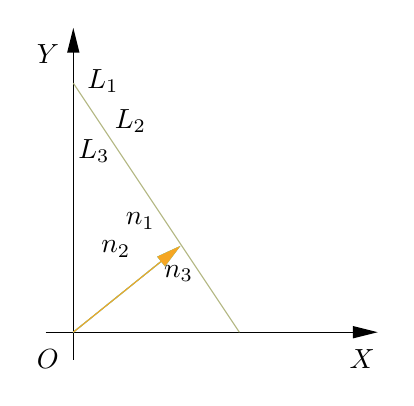
\begin{tikzpicture}[x=0.75pt,y=0.75pt,yscale=-1,xscale=1]
    %uncomment if require: \path (0,310); %set diagram left start at 0, and has height of 310
    
    %Straight Lines [id:da35662438044042455] 
    \draw    (173.33,173.33) -- (173.33,146.67) -- (173.33,120) -- (173.33,93.33) -- (173.33,66.67) -- (173.33,40) -- (173.33,15.33) ;
    \draw [shift={(173.33,13.33)}, rotate = 90] [fill={rgb, 255:red, 0; green, 0; blue, 0 }  ][line width=0.08]  [draw opacity=0] (12,-3) -- (0,0) -- (12,3) -- cycle    ;
    %Straight Lines [id:da4695778774553647] 
    \draw    (160,160) -- (186.67,160) -- (213.33,160) -- (240,160) -- (266.67,160) -- (293.33,160) -- (318,160) ;
    \draw [shift={(320,160)}, rotate = 180] [fill={rgb, 255:red, 0; green, 0; blue, 0 }  ][line width=0.08]  [draw opacity=0] (12,-3) -- (0,0) -- (12,3) -- cycle    ;
    %Straight Lines [id:da6388562181423141] 
    \draw [color={rgb, 255:red, 155; green, 155; blue, 155 }  ,draw opacity=1 ][fill={rgb, 255:red, 155; green, 155; blue, 155 }  ,fill opacity=1 ]   (173.33,160) -- (223.4,119.65) ;
    \draw [shift={(224.96,118.4)}, rotate = 141.14] [fill={rgb, 255:red, 155; green, 155; blue, 155 }  ,fill opacity=1 ][line width=0.08]  [draw opacity=0] (12,-3) -- (0,0) -- (12,3) -- cycle    ;
    %Straight Lines [id:da25970309226664057] 
    \draw [color={rgb, 255:red, 80; green, 227; blue, 194 }  ,draw opacity=1 ][fill={rgb, 255:red, 155; green, 155; blue, 155 }  ,fill opacity=1 ]   (173.33,160) -- (223.4,119.65) ;
    \draw [shift={(224.96,118.4)}, rotate = 141.14] [fill={rgb, 255:red, 80; green, 227; blue, 194 }  ,fill opacity=1 ][line width=0.08]  [draw opacity=0] (12,-3) -- (0,0) -- (12,3) -- cycle    ;
    %Straight Lines [id:da9422793466632897] 
    \draw [color={rgb, 255:red, 245; green, 166; blue, 35 }  ,draw opacity=1 ][fill={rgb, 255:red, 155; green, 155; blue, 155 }  ,fill opacity=1 ]   (173.33,160) -- (223.4,119.65) ;
    \draw [shift={(224.96,118.4)}, rotate = 141.14] [fill={rgb, 255:red, 245; green, 166; blue, 35 }  ,fill opacity=1 ][line width=0.08]  [draw opacity=0] (12,-3) -- (0,0) -- (12,3) -- cycle    ;
    %Straight Lines [id:da029423082616190976] 
    \draw [color={rgb, 255:red, 155; green, 155; blue, 155 }  ,draw opacity=0.35 ][fill={rgb, 255:red, 155; green, 155; blue, 155 }  ,fill opacity=1 ]   (173.33,40) -- (253.33,160) ;
    %Straight Lines [id:da9204169647154299] 
    \draw [color={rgb, 255:red, 80; green, 227; blue, 194 }  ,draw opacity=0.35 ][fill={rgb, 255:red, 155; green, 155; blue, 155 }  ,fill opacity=1 ]   (173.33,40) -- (253.33,160) ;
    %Straight Lines [id:da8049491803274635] 
    \draw [color={rgb, 255:red, 245; green, 166; blue, 35 }  ,draw opacity=0.35 ][fill={rgb, 255:red, 155; green, 155; blue, 155 }  ,fill opacity=1 ]   (173.33,40) -- (253.33,160) ;
    
    % Text Node
    \draw (312.88,172.78) node   [align=left] {\begin{minipage}[lt]{9.68pt}\setlength\topsep{0pt}
    $\displaystyle X$
    \end{minipage}};
    % Text Node
    \draw (164.13,26.11) node   [align=left] {\begin{minipage}[lt]{12.51pt}\setlength\topsep{0pt}
    $\displaystyle Y$
    \end{minipage}};
    % Text Node
    \draw (164.15,172.78) node   [align=left] {\begin{minipage}[lt]{12.49pt}\setlength\topsep{0pt}
    $\displaystyle O$
    \end{minipage}};
    % Text Node
    \draw (206.27,106.42) node   [align=left] {\begin{minipage}[lt]{11.42pt}\setlength\topsep{0pt}
    $\displaystyle \boldsymbol{n}_{1}$
    \end{minipage}};
    % Text Node
    \draw (194.43,119.93) node   [align=left] {\begin{minipage}[lt]{11.42pt}\setlength\topsep{0pt}
    $\displaystyle \boldsymbol{n}_{2}$
    \end{minipage}};
    % Text Node
    \draw (224.67,131.92) node   [align=left] {\begin{minipage}[lt]{11.42pt}\setlength\topsep{0pt}
    $\displaystyle \boldsymbol{n}_{3}$
    \end{minipage}};
    % Text Node
    \draw (189.84,38.86) node   [align=left] {\begin{minipage}[lt]{14.58pt}\setlength\topsep{0pt}
    $\displaystyle L_{1}$
    \end{minipage}};
    % Text Node
    \draw (203.04,58.46) node   [align=left] {\begin{minipage}[lt]{14.58pt}\setlength\topsep{0pt}
    $\displaystyle L_{2}$
    \end{minipage}};
    % Text Node
    \draw (185.44,72.86) node   [align=left] {\begin{minipage}[lt]{14.58pt}\setlength\topsep{0pt}
    $\displaystyle L_{3}$
    \end{minipage}};
    
    
    \end{tikzpicture}
    

    }
    \subfigure[scale=.9][$r(\vb*{A})=2\neq r(\bar{\vb*{A}})=3$]{
        

\tikzset{every picture/.style={line width=0.75pt}} %set default line width to 0.75pt        

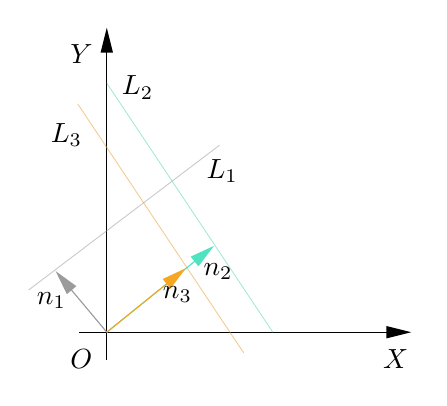
\begin{tikzpicture}[x=0.75pt,y=0.75pt,yscale=-1,xscale=1]
%uncomment if require: \path (0,310); %set diagram left start at 0, and has height of 310

%Straight Lines [id:da07430350371938887] 
\draw    (193.33,200.55) -- (193.33,173.89) -- (193.33,147.22) -- (193.33,120.55) -- (193.33,93.89) -- (193.33,67.22) -- (193.33,42.55) ;
\draw [shift={(193.33,40.55)}, rotate = 90] [fill={rgb, 255:red, 0; green, 0; blue, 0 }  ][line width=0.08]  [draw opacity=0] (12,-3) -- (0,0) -- (12,3) -- cycle    ;
%Straight Lines [id:da47102922798219593] 
\draw    (180,187.22) -- (206.67,187.22) -- (233.33,187.22) -- (260,187.22) -- (286.67,187.22) -- (313.33,187.22) -- (338,187.22) ;
\draw [shift={(340,187.22)}, rotate = 180] [fill={rgb, 255:red, 0; green, 0; blue, 0 }  ][line width=0.08]  [draw opacity=0] (12,-3) -- (0,0) -- (12,3) -- cycle    ;
%Straight Lines [id:da28590180102079454] 
\draw [color={rgb, 255:red, 155; green, 155; blue, 155 }  ,draw opacity=1 ][fill={rgb, 255:red, 155; green, 155; blue, 155 }  ,fill opacity=1 ]   (193.33,187.22) -- (169.95,159.3) ;
\draw [shift={(168.67,157.77)}, rotate = 50.05] [fill={rgb, 255:red, 155; green, 155; blue, 155 }  ,fill opacity=1 ][line width=0.08]  [draw opacity=0] (12,-3) -- (0,0) -- (12,3) -- cycle    ;
%Straight Lines [id:da7422637416191584] 
\draw [color={rgb, 255:red, 80; green, 227; blue, 194 }  ,draw opacity=1 ][fill={rgb, 255:red, 155; green, 155; blue, 155 }  ,fill opacity=1 ]   (193.33,187.22) -- (243.4,146.87) ;
\draw [shift={(244.96,145.62)}, rotate = 141.14] [fill={rgb, 255:red, 80; green, 227; blue, 194 }  ,fill opacity=1 ][line width=0.08]  [draw opacity=0] (12,-3) -- (0,0) -- (12,3) -- cycle    ;
%Straight Lines [id:da46524637945955694] 
\draw [color={rgb, 255:red, 245; green, 166; blue, 35 }  ,draw opacity=1 ][fill={rgb, 255:red, 155; green, 155; blue, 155 }  ,fill opacity=1 ]   (193.33,187.22) -- (229.91,157.62) ;
\draw [shift={(231.47,156.37)}, rotate = 141.02] [fill={rgb, 255:red, 245; green, 166; blue, 35 }  ,fill opacity=1 ][line width=0.08]  [draw opacity=0] (12,-3) -- (0,0) -- (12,3) -- cycle    ;
%Straight Lines [id:da7389989440306435] 
\draw [color={rgb, 255:red, 155; green, 155; blue, 155 }  ,draw opacity=0.35 ][fill={rgb, 255:red, 155; green, 155; blue, 155 }  ,fill opacity=1 ]   (247.67,97.1) -- (155.67,166.89) ;
%Straight Lines [id:da3172580725565546] 
\draw [color={rgb, 255:red, 80; green, 227; blue, 194 }  ,draw opacity=0.35 ][fill={rgb, 255:red, 155; green, 155; blue, 155 }  ,fill opacity=1 ]   (193.33,67.22) -- (224.93,114.61) -- (273.33,187.22) ;
%Straight Lines [id:da20689843266136476] 
\draw [color={rgb, 255:red, 245; green, 166; blue, 35 }  ,draw opacity=0.35 ][fill={rgb, 255:red, 155; green, 155; blue, 155 }  ,fill opacity=1 ]   (179.33,77.22) -- (210.97,124.68) -- (259.33,197.22) ;

% Text Node
\draw (332.88,200) node   [align=left] {\begin{minipage}[lt]{9.68pt}\setlength\topsep{0pt}
$\displaystyle X$
\end{minipage}};
% Text Node
\draw (184.13,53.33) node   [align=left] {\begin{minipage}[lt]{12.51pt}\setlength\topsep{0pt}
$\displaystyle Y$
\end{minipage}};
% Text Node
\draw (184.15,200) node   [align=left] {\begin{minipage}[lt]{12.49pt}\setlength\topsep{0pt}
$\displaystyle O$
\end{minipage}};
% Text Node
\draw (167.27,171.98) node   [align=left] {\begin{minipage}[lt]{11.42pt}\setlength\topsep{0pt}
$\displaystyle \boldsymbol{n}_{1}$
\end{minipage}};
% Text Node
\draw (247.6,157.79) node   [align=left] {\begin{minipage}[lt]{11.42pt}\setlength\topsep{0pt}
$\displaystyle \boldsymbol{n}_{2}$
\end{minipage}};
% Text Node
\draw (228,169.14) node   [align=left] {\begin{minipage}[lt]{11.42pt}\setlength\topsep{0pt}
$\displaystyle \boldsymbol{n}_{3}$
\end{minipage}};
% Text Node
\draw (251.17,109.41) node   [align=left] {\begin{minipage}[lt]{14.58pt}\setlength\topsep{0pt}
$\displaystyle L_{1}$
\end{minipage}};
% Text Node
\draw (210.37,69.35) node   [align=left] {\begin{minipage}[lt]{14.58pt}\setlength\topsep{0pt}
$\displaystyle L_{2}$
\end{minipage}};
% Text Node
\draw (176.11,92.08) node   [align=left] {\begin{minipage}[lt]{14.58pt}\setlength\topsep{0pt}
$\displaystyle L_{3}$
\end{minipage}};


\end{tikzpicture}

    }
    \subfigure[scale=.9][$r(\vb*{A})=2\neq r(\bar{\vb*{A}})=3$]{
        

\tikzset{every picture/.style={line width=0.75pt}} %set default line width to 0.75pt        

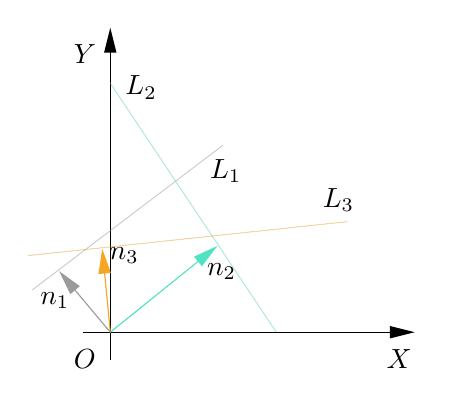
\begin{tikzpicture}[x=0.75pt,y=0.75pt,yscale=-1,xscale=1]
%uncomment if require: \path (0,310); %set diagram left start at 0, and has height of 310

%Straight Lines [id:da6776809984537686] 
\draw    (193.33,200.55) -- (193.33,173.89) -- (193.33,147.22) -- (193.33,120.55) -- (193.33,93.89) -- (193.33,67.22) -- (193.33,42.55) ;
\draw [shift={(193.33,40.55)}, rotate = 90] [fill={rgb, 255:red, 0; green, 0; blue, 0 }  ][line width=0.08]  [draw opacity=0] (12,-3) -- (0,0) -- (12,3) -- cycle    ;
%Straight Lines [id:da48375060583244545] 
\draw    (180,187.22) -- (206.67,187.22) -- (233.33,187.22) -- (260,187.22) -- (286.67,187.22) -- (313.33,187.22) -- (338,187.22) ;
\draw [shift={(340,187.22)}, rotate = 180] [fill={rgb, 255:red, 0; green, 0; blue, 0 }  ][line width=0.08]  [draw opacity=0] (12,-3) -- (0,0) -- (12,3) -- cycle    ;
%Straight Lines [id:da4050036301008375] 
\draw [color={rgb, 255:red, 155; green, 155; blue, 155 }  ,draw opacity=1 ][fill={rgb, 255:red, 155; green, 155; blue, 155 }  ,fill opacity=1 ]   (193.33,187.22) -- (169.95,159.3) ;
\draw [shift={(168.67,157.77)}, rotate = 50.05] [fill={rgb, 255:red, 155; green, 155; blue, 155 }  ,fill opacity=1 ][line width=0.08]  [draw opacity=0] (12,-3) -- (0,0) -- (12,3) -- cycle    ;
%Straight Lines [id:da8143366333117024] 
\draw [color={rgb, 255:red, 80; green, 227; blue, 194 }  ,draw opacity=1 ][fill={rgb, 255:red, 155; green, 155; blue, 155 }  ,fill opacity=1 ]   (193.33,187.22) -- (243.4,146.87) ;
\draw [shift={(244.96,145.62)}, rotate = 141.14] [fill={rgb, 255:red, 80; green, 227; blue, 194 }  ,fill opacity=1 ][line width=0.08]  [draw opacity=0] (12,-3) -- (0,0) -- (12,3) -- cycle    ;
%Straight Lines [id:da12025340326131895] 
\draw [color={rgb, 255:red, 245; green, 166; blue, 35 }  ,draw opacity=1 ][fill={rgb, 255:red, 155; green, 155; blue, 155 }  ,fill opacity=1 ]   (193.33,187.22) -- (189.66,148.96) ;
\draw [shift={(189.47,146.97)}, rotate = 84.51] [fill={rgb, 255:red, 245; green, 166; blue, 35 }  ,fill opacity=1 ][line width=0.08]  [draw opacity=0] (12,-3) -- (0,0) -- (12,3) -- cycle    ;
%Straight Lines [id:da03970357990115825] 
\draw [color={rgb, 255:red, 155; green, 155; blue, 155 }  ,draw opacity=0.35 ][fill={rgb, 255:red, 155; green, 155; blue, 155 }  ,fill opacity=1 ]   (247.67,97.1) -- (155.67,166.89) ;
%Straight Lines [id:da32766536204692986] 
\draw [color={rgb, 255:red, 80; green, 227; blue, 194 }  ,draw opacity=0.35 ][fill={rgb, 255:red, 155; green, 155; blue, 155 }  ,fill opacity=1 ]   (193.33,67.22) -- (224.93,114.61) -- (273.33,187.22) ;
%Straight Lines [id:da44792737596538945] 
\draw [color={rgb, 255:red, 245; green, 166; blue, 35 }  ,draw opacity=0.35 ][fill={rgb, 255:red, 155; green, 155; blue, 155 }  ,fill opacity=1 ]   (153.8,150.3) -- (307.47,133.97) ;

% Text Node
\draw (332.88,200) node   [align=left] {\begin{minipage}[lt]{9.68pt}\setlength\topsep{0pt}
$\displaystyle X$
\end{minipage}};
% Text Node
\draw (184.13,53.33) node   [align=left] {\begin{minipage}[lt]{12.51pt}\setlength\topsep{0pt}
$\displaystyle Y$
\end{minipage}};
% Text Node
\draw (184.15,200) node   [align=left] {\begin{minipage}[lt]{12.49pt}\setlength\topsep{0pt}
$\displaystyle O$
\end{minipage}};
% Text Node
\draw (167.27,171.98) node   [align=left] {\begin{minipage}[lt]{11.42pt}\setlength\topsep{0pt}
$\displaystyle \boldsymbol{n}_{1}$
\end{minipage}};
% Text Node
\draw (247.6,157.79) node   [align=left] {\begin{minipage}[lt]{11.42pt}\setlength\topsep{0pt}
$\displaystyle \boldsymbol{n}_{2}$
\end{minipage}};
% Text Node
\draw (200.67,150.48) node   [align=left] {\begin{minipage}[lt]{11.42pt}\setlength\topsep{0pt}
$\displaystyle \boldsymbol{n}_{3}$
\end{minipage}};
% Text Node
\draw (251.17,109.41) node   [align=left] {\begin{minipage}[lt]{14.58pt}\setlength\topsep{0pt}
$\displaystyle L_{1}$
\end{minipage}};
% Text Node
\draw (210.37,69.35) node   [align=left] {\begin{minipage}[lt]{14.58pt}\setlength\topsep{0pt}
$\displaystyle L_{2}$
\end{minipage}};
% Text Node
\draw (305.44,123.41) node   [align=left] {\begin{minipage}[lt]{14.58pt}\setlength\topsep{0pt}
$\displaystyle L_{3}$
\end{minipage}};


\end{tikzpicture}

    }
    \subfigure[scale=.9][$r(\vb*{A})=1\neq r(\bar{\vb*{A}})=2$]{
        

\tikzset{every picture/.style={line width=0.75pt}} %set default line width to 0.75pt        

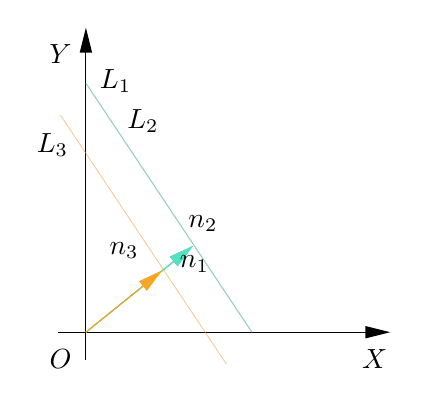
\begin{tikzpicture}[x=0.75pt,y=0.75pt,yscale=-1,xscale=1]
%uncomment if require: \path (0,310); %set diagram left start at 0, and has height of 310

%Straight Lines [id:da16102372571387868] 
\draw    (173.33,173.33) -- (173.33,146.67) -- (173.33,120) -- (173.33,93.33) -- (173.33,66.67) -- (173.33,40) -- (173.33,15.33) ;
\draw [shift={(173.33,13.33)}, rotate = 90] [fill={rgb, 255:red, 0; green, 0; blue, 0 }  ][line width=0.08]  [draw opacity=0] (12,-3) -- (0,0) -- (12,3) -- cycle    ;
%Straight Lines [id:da7856232306084785] 
\draw    (160,160) -- (186.67,160) -- (213.33,160) -- (240,160) -- (266.67,160) -- (293.33,160) -- (318,160) ;
\draw [shift={(320,160)}, rotate = 180] [fill={rgb, 255:red, 0; green, 0; blue, 0 }  ][line width=0.08]  [draw opacity=0] (12,-3) -- (0,0) -- (12,3) -- cycle    ;
%Straight Lines [id:da31218072017713916] 
\draw [color={rgb, 255:red, 155; green, 155; blue, 155 }  ,draw opacity=1 ][fill={rgb, 255:red, 155; green, 155; blue, 155 }  ,fill opacity=1 ]   (173.33,160) -- (223.4,119.65) ;
\draw [shift={(224.96,118.4)}, rotate = 141.14] [fill={rgb, 255:red, 155; green, 155; blue, 155 }  ,fill opacity=1 ][line width=0.08]  [draw opacity=0] (12,-3) -- (0,0) -- (12,3) -- cycle    ;
%Straight Lines [id:da5889295414997142] 
\draw [color={rgb, 255:red, 80; green, 227; blue, 194 }  ,draw opacity=1 ][fill={rgb, 255:red, 155; green, 155; blue, 155 }  ,fill opacity=1 ]   (173.33,160) -- (223.4,119.65) ;
\draw [shift={(224.96,118.4)}, rotate = 141.14] [fill={rgb, 255:red, 80; green, 227; blue, 194 }  ,fill opacity=1 ][line width=0.08]  [draw opacity=0] (12,-3) -- (0,0) -- (12,3) -- cycle    ;
%Straight Lines [id:da748720455222248] 
\draw [color={rgb, 255:red, 245; green, 166; blue, 35 }  ,draw opacity=1 ][fill={rgb, 255:red, 155; green, 155; blue, 155 }  ,fill opacity=1 ]   (173.33,160) -- (208.58,131.43) ;
\draw [shift={(210.13,130.17)}, rotate = 140.97] [fill={rgb, 255:red, 245; green, 166; blue, 35 }  ,fill opacity=1 ][line width=0.08]  [draw opacity=0] (12,-3) -- (0,0) -- (12,3) -- cycle    ;
%Straight Lines [id:da3413533559265185] 
\draw [color={rgb, 255:red, 155; green, 155; blue, 155 }  ,draw opacity=0.35 ][fill={rgb, 255:red, 155; green, 155; blue, 155 }  ,fill opacity=1 ]   (173.33,40) -- (253.33,160) ;
%Straight Lines [id:da5680956214783399] 
\draw [color={rgb, 255:red, 80; green, 227; blue, 194 }  ,draw opacity=0.35 ][fill={rgb, 255:red, 155; green, 155; blue, 155 }  ,fill opacity=1 ]   (173.33,40) -- (253.33,160) ;
%Straight Lines [id:da5035499664456724] 
\draw [color={rgb, 255:red, 245; green, 166; blue, 35 }  ,draw opacity=0.35 ][fill={rgb, 255:red, 155; green, 155; blue, 155 }  ,fill opacity=1 ]   (161,55.33) -- (241,175.33) ;

% Text Node
\draw (312.88,172.78) node   [align=left] {\begin{minipage}[lt]{9.68pt}\setlength\topsep{0pt}
$\displaystyle X$
\end{minipage}};
% Text Node
\draw (164.13,26.11) node   [align=left] {\begin{minipage}[lt]{12.51pt}\setlength\topsep{0pt}
$\displaystyle Y$
\end{minipage}};
% Text Node
\draw (164.15,172.78) node   [align=left] {\begin{minipage}[lt]{12.49pt}\setlength\topsep{0pt}
$\displaystyle O$
\end{minipage}};
% Text Node
\draw (226.23,127.16) node   [align=left] {\begin{minipage}[lt]{11.42pt}\setlength\topsep{0pt}
$\displaystyle \boldsymbol{n}_{1}$
\end{minipage}};
% Text Node
\draw (230.36,107.83) node   [align=left] {\begin{minipage}[lt]{11.42pt}\setlength\topsep{0pt}
$\displaystyle \boldsymbol{n}_{2}$
\end{minipage}};
% Text Node
\draw (192.33,120.59) node   [align=left] {\begin{minipage}[lt]{11.42pt}\setlength\topsep{0pt}
$\displaystyle \boldsymbol{n}_{3}$
\end{minipage}};
% Text Node
\draw (189.84,38.86) node   [align=left] {\begin{minipage}[lt]{14.58pt}\setlength\topsep{0pt}
$\displaystyle L_{1}$
\end{minipage}};
% Text Node
\draw (203.04,58.46) node   [align=left] {\begin{minipage}[lt]{14.58pt}\setlength\topsep{0pt}
$\displaystyle L_{2}$
\end{minipage}};
% Text Node
\draw (159.44,69.86) node   [align=left] {\begin{minipage}[lt]{14.58pt}\setlength\topsep{0pt}
$\displaystyle L_{3}$
\end{minipage}};


\end{tikzpicture}

    }
    \subfigure[scale=.9][$r(\vb*{A})=1\neq r(\bar{\vb*{A}})=3$]{
        

\tikzset{every picture/.style={line width=0.75pt}} %set default line width to 0.75pt        

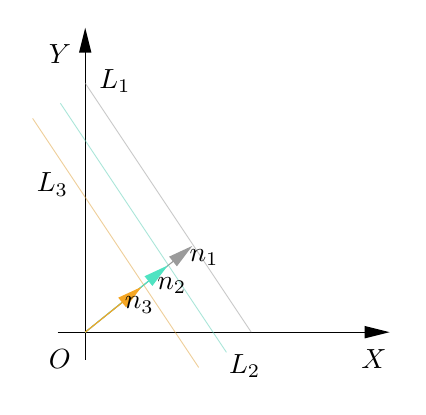
\begin{tikzpicture}[x=0.75pt,y=0.75pt,yscale=-1,xscale=1]
%uncomment if require: \path (0,310); %set diagram left start at 0, and has height of 310

%Straight Lines [id:da2550131407857221] 
\draw    (173.33,173.33) -- (173.33,146.67) -- (173.33,120) -- (173.33,93.33) -- (173.33,66.67) -- (173.33,40) -- (173.33,15.33) ;
\draw [shift={(173.33,13.33)}, rotate = 90] [fill={rgb, 255:red, 0; green, 0; blue, 0 }  ][line width=0.08]  [draw opacity=0] (12,-3) -- (0,0) -- (12,3) -- cycle    ;
%Straight Lines [id:da7379015741945953] 
\draw    (160,160) -- (186.67,160) -- (213.33,160) -- (240,160) -- (266.67,160) -- (293.33,160) -- (318,160) ;
\draw [shift={(320,160)}, rotate = 180] [fill={rgb, 255:red, 0; green, 0; blue, 0 }  ][line width=0.08]  [draw opacity=0] (12,-3) -- (0,0) -- (12,3) -- cycle    ;
%Straight Lines [id:da302067719857668] 
\draw [color={rgb, 255:red, 155; green, 155; blue, 155 }  ,draw opacity=1 ][fill={rgb, 255:red, 155; green, 155; blue, 155 }  ,fill opacity=1 ]   (173.33,160) -- (223.4,119.65) ;
\draw [shift={(224.96,118.4)}, rotate = 141.14] [fill={rgb, 255:red, 155; green, 155; blue, 155 }  ,fill opacity=1 ][line width=0.08]  [draw opacity=0] (12,-3) -- (0,0) -- (12,3) -- cycle    ;
%Straight Lines [id:da17370985345603196] 
\draw [color={rgb, 255:red, 80; green, 227; blue, 194 }  ,draw opacity=1 ][fill={rgb, 255:red, 155; green, 155; blue, 155 }  ,fill opacity=1 ]   (173.33,160) -- (211.58,129.09) ;
\draw [shift={(213.13,127.83)}, rotate = 141.05] [fill={rgb, 255:red, 80; green, 227; blue, 194 }  ,fill opacity=1 ][line width=0.08]  [draw opacity=0] (12,-3) -- (0,0) -- (12,3) -- cycle    ;
%Straight Lines [id:da8271888135621248] 
\draw [color={rgb, 255:red, 245; green, 166; blue, 35 }  ,draw opacity=1 ][fill={rgb, 255:red, 155; green, 155; blue, 155 }  ,fill opacity=1 ]   (173.33,160) -- (198.91,139.42) ;
\draw [shift={(200.47,138.17)}, rotate = 141.18] [fill={rgb, 255:red, 245; green, 166; blue, 35 }  ,fill opacity=1 ][line width=0.08]  [draw opacity=0] (12,-3) -- (0,0) -- (12,3) -- cycle    ;
%Straight Lines [id:da3682069340578269] 
\draw [color={rgb, 255:red, 155; green, 155; blue, 155 }  ,draw opacity=0.35 ][fill={rgb, 255:red, 155; green, 155; blue, 155 }  ,fill opacity=1 ]   (173.33,40) -- (253.33,160) ;
%Straight Lines [id:da6225208131903259] 
\draw [color={rgb, 255:red, 80; green, 227; blue, 194 }  ,draw opacity=0.35 ][fill={rgb, 255:red, 155; green, 155; blue, 155 }  ,fill opacity=1 ]   (161.33,49.67) -- (201.91,110.54) -- (241.33,169.67) ;
%Straight Lines [id:da833082804623273] 
\draw [color={rgb, 255:red, 245; green, 166; blue, 35 }  ,draw opacity=0.35 ][fill={rgb, 255:red, 155; green, 155; blue, 155 }  ,fill opacity=1 ]   (148,57) -- (228,177) ;

% Text Node
\draw (312.88,172.78) node   [align=left] {\begin{minipage}[lt]{9.68pt}\setlength\topsep{0pt}
$\displaystyle X$
\end{minipage}};
% Text Node
\draw (164.13,26.11) node   [align=left] {\begin{minipage}[lt]{12.51pt}\setlength\topsep{0pt}
$\displaystyle Y$
\end{minipage}};
% Text Node
\draw (164.15,172.78) node   [align=left] {\begin{minipage}[lt]{12.49pt}\setlength\topsep{0pt}
$\displaystyle O$
\end{minipage}};
% Text Node
\draw (231.23,124.16) node   [align=left] {\begin{minipage}[lt]{11.42pt}\setlength\topsep{0pt}
$\displaystyle \boldsymbol{n}_{1}$
\end{minipage}};
% Text Node
\draw (215.69,137.49) node   [align=left] {\begin{minipage}[lt]{11.42pt}\setlength\topsep{0pt}
$\displaystyle \boldsymbol{n}_{2}$
\end{minipage}};
% Text Node
\draw (200,146.92) node   [align=left] {\begin{minipage}[lt]{11.42pt}\setlength\topsep{0pt}
$\displaystyle \boldsymbol{n}_{3}$
\end{minipage}};
% Text Node
\draw (189.84,38.86) node   [align=left] {\begin{minipage}[lt]{14.58pt}\setlength\topsep{0pt}
$\displaystyle L_{1}$
\end{minipage}};
% Text Node
\draw (252.37,176.46) node   [align=left] {\begin{minipage}[lt]{14.58pt}\setlength\topsep{0pt}
$\displaystyle L_{2}$
\end{minipage}};
% Text Node
\draw (159.77,88.86) node   [align=left] {\begin{minipage}[lt]{14.58pt}\setlength\topsep{0pt}
$\displaystyle L_{3}$
\end{minipage}};


\end{tikzpicture}

    }
    \caption{}
    \label{xxfczjiheyy}
\end{figure}

\subsubsection{平面与平面之间的位置关系}

\begin{theorem}[平面位置关系]
    对 $\vb*{Ax}=\vb*{b}$ 方程组,若方程组有解,则 $\rank(\vb*{A},\vb*{b})=\rank\vb*{A}=3$, 并且 
    $$
    \begin{cases}
        \text{唯一解: 三个平面互不重合且相交于一点, 如图 \ref{mianmiangx}(a), } \rank\vb*{A}=\rank\bar{\vb*{A}}=3\\ 
        \text{无穷多解: }\begin{cases}
            \text{三平面相交于一条直线, 如图 \ref{mianmiangx}(b), }\rank\vb*{A}=\rank\bar{\vb*{A}}=2\\ 
            \text{两平面重叠, 并与第三平面相交于一条直线, 如图 \ref{mianmiangx}(c), }\rank\vb*{A}=\rank\bar{\vb*{A}}=2\\ 
            \text{三平面互相重叠, 如图 \ref{mianmiangx}(d), }\rank\vb*{A}=\rank\bar{\vb*{A}}=1
        \end{cases}\\ 
        \text{无解: }\begin{cases}
            \text{两平面平行, 并与第三平面相交, 如图 \ref{mianmiangx}(e), }\rank\vb*{A}=2\neq\rank\bar{\vb*{A}}=3\\ 
            \text{三平面两两相交于一条直线, 如图 \ref{mianmiangx}(f), }\rank\vb*{A}=2\neq\rank\bar{\vb*{A}}=3\\ 
            \text{两平面重叠, 并与第三平面平行, 如图 \ref{mianmiangx}(g), }\rank\vb*{A}=1\neq\rank\bar{\vb*{A}}=2\\ 
            \text{三平面互不重叠, 且相互平行, 如图 \ref{mianmiangx}(h), }\rank\vb*{A}=1\neq\rank\bar{\vb*{A}}=3\\ 
        \end{cases}
    \end{cases}
    $$
\end{theorem}

\begin{figure}[H]
    \centering
    \subfigure[scale=.9][$r(\vb{A})=r\qty(\bar{\vb{A}})=3$有唯一解]{


    \tikzset{every picture/.style={line width=0.75pt}} %set default line width to 0.75pt        

    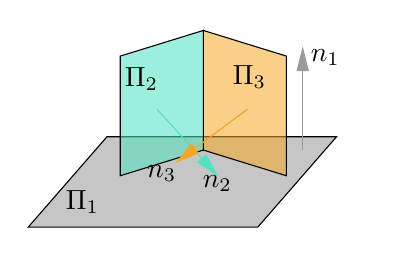
\begin{tikzpicture}[x=0.75pt,y=0.75pt,yscale=-1,xscale=1]
    %uncomment if require: \path (0,310); %set diagram left start at 0, and has height of 310
    
    %Shape: Parallelogram [id:dp13681346255413596] 
    \draw  [fill={rgb, 255:red, 155; green, 155; blue, 155 }  ,fill opacity=0.57 ] (144.51,122.2) -- (255.12,122.2) -- (217.17,165.76) -- (106.56,165.76) -- cycle ;
    %Shape: Parallelogram [id:dp8859917931291947] 
    \draw  [fill={rgb, 255:red, 245; green, 166; blue, 35 }  ,fill opacity=0.54 ] (230.92,83.36) -- (230.92,141) -- (190.92,128.64) -- (190.92,71) -- cycle ;
    %Shape: Parallelogram [id:dp8993649334283396] 
    \draw  [fill={rgb, 255:red, 80; green, 227; blue, 194 }  ,fill opacity=0.56 ] (150.92,141) -- (150.92,83.36) -- (190.92,71) -- (190.92,128.64) -- cycle ;
    %Straight Lines [id:da9705336789841945] 
    \draw [color={rgb, 255:red, 155; green, 155; blue, 155 }  ,draw opacity=1 ][fill={rgb, 255:red, 155; green, 155; blue, 155 }  ,fill opacity=1 ]   (238.8,128.6) -- (238.8,80.6) ;
    \draw [shift={(238.8,78.6)}, rotate = 90] [fill={rgb, 255:red, 155; green, 155; blue, 155 }  ,fill opacity=1 ][line width=0.08]  [draw opacity=0] (12,-3) -- (0,0) -- (12,3) -- cycle    ;
    %Straight Lines [id:da22520091261193587] 
    \draw [color={rgb, 255:red, 80; green, 227; blue, 194 }  ,draw opacity=1 ][fill={rgb, 255:red, 155; green, 155; blue, 155 }  ,fill opacity=1 ]   (168.56,108.96) -- (196.81,139.88) ;
    \draw [shift={(198.16,141.36)}, rotate = 227.59] [fill={rgb, 255:red, 80; green, 227; blue, 194 }  ,fill opacity=1 ][line width=0.08]  [draw opacity=0] (12,-3) -- (0,0) -- (12,3) -- cycle    ;
    %Straight Lines [id:da36864291238566915] 
    \draw [color={rgb, 255:red, 245; green, 166; blue, 35 }  ,draw opacity=1 ][fill={rgb, 255:red, 155; green, 155; blue, 155 }  ,fill opacity=1 ]   (212.16,108.96) -- (178.96,133.76) ;
    \draw [shift={(177.36,134.96)}, rotate = 323.24] [fill={rgb, 255:red, 245; green, 166; blue, 35 }  ,fill opacity=1 ][line width=0.08]  [draw opacity=0] (12,-3) -- (0,0) -- (12,3) -- cycle    ;
    
    % Text Node
    \draw (136.44,153.78) node   [align=left] {\begin{minipage}[lt]{17.57pt}\setlength\topsep{0pt}
    $\displaystyle \Pi _{1}$
    \end{minipage}};
    % Text Node
    \draw (216.84,93.38) node   [align=left] {\begin{minipage}[lt]{17.57pt}\setlength\topsep{0pt}
    $\displaystyle \Pi _{3}$
    \end{minipage}};
    % Text Node
    \draw (164.84,94.58) node   [align=left] {\begin{minipage}[lt]{17.57pt}\setlength\topsep{0pt}
    $\displaystyle \Pi _{2}$
    \end{minipage}};
    % Text Node
    \draw (256.44,75.78) node   [align=left] {\begin{minipage}[lt]{17.57pt}\setlength\topsep{0pt}
    $ $
    \end{minipage}};
    % Text Node
    \draw (250.3,84.02) node   [align=left] {\begin{minipage}[lt]{11.42pt}\setlength\topsep{0pt}
    $\displaystyle \boldsymbol{n}_{1}$
    \end{minipage}};
    % Text Node
    \draw (198.3,144.82) node   [align=left] {\begin{minipage}[lt]{11.42pt}\setlength\topsep{0pt}
    $\displaystyle \boldsymbol{n}_{2}$
    \end{minipage}};
    % Text Node
    \draw (171.5,140.02) node   [align=left] {\begin{minipage}[lt]{11.42pt}\setlength\topsep{0pt}
    $\displaystyle \boldsymbol{n}_{3}$
    \end{minipage}};
    
    
    \end{tikzpicture}
    }
    \subfigure[scale=.9][$r(\vb{A})=r\qty(\bar{\vb{A}})=2$ 有无穷解]{


    \tikzset{every picture/.style={line width=0.75pt}} %set default line width to 0.75pt        

    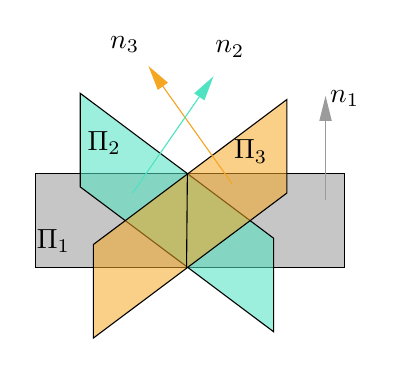
\begin{tikzpicture}[x=0.75pt,y=0.75pt,yscale=-1,xscale=1]
    %uncomment if require: \path (0,310); %set diagram left start at 0, and has height of 310
    
    %Shape: Parallelogram [id:dp3516738443909617] 
    \draw  [fill={rgb, 255:red, 155; green, 155; blue, 155 }  ,fill opacity=0.57 ] (103.59,128.01) -- (252.15,128.01) -- (252.15,173.17) -- (103.59,173.17) -- cycle ;
    %Shape: Parallelogram [id:dp7310377507468195] 
    \draw  [fill={rgb, 255:red, 80; green, 227; blue, 194 }  ,fill opacity=0.56 ] (218.14,159.17) -- (218.14,204.24) -- (124.94,134.41) -- (124.94,89.33) -- cycle ;
    %Shape: Parallelogram [id:dp31987316522235787] 
    \draw  [fill={rgb, 255:red, 245; green, 166; blue, 35 }  ,fill opacity=0.54 ] (224.47,92.33) -- (224.47,137.41) -- (131.28,207.24) -- (131.28,162.17) -- cycle ;
    %Straight Lines [id:da2436964117379603] 
    \draw [color={rgb, 255:red, 155; green, 155; blue, 155 }  ,draw opacity=1 ][fill={rgb, 255:red, 155; green, 155; blue, 155 }  ,fill opacity=1 ]   (243.13,140.6) -- (243.13,92.6) ;
    \draw [shift={(243.13,90.6)}, rotate = 90] [fill={rgb, 255:red, 155; green, 155; blue, 155 }  ,fill opacity=1 ][line width=0.08]  [draw opacity=0] (12,-3) -- (0,0) -- (12,3) -- cycle    ;
    %Straight Lines [id:da777468594508129] 
    \draw [color={rgb, 255:red, 245; green, 166; blue, 35 }  ,draw opacity=1 ][fill={rgb, 255:red, 155; green, 155; blue, 155 }  ,fill opacity=1 ]   (198.16,132.96) -- (158.96,77.8) ;
    \draw [shift={(157.8,76.17)}, rotate = 54.6] [fill={rgb, 255:red, 245; green, 166; blue, 35 }  ,fill opacity=1 ][line width=0.08]  [draw opacity=0] (12,-3) -- (0,0) -- (12,3) -- cycle    ;
    %Straight Lines [id:da6986337147617758] 
    \draw [color={rgb, 255:red, 80; green, 227; blue, 194 }  ,draw opacity=1 ][fill={rgb, 255:red, 155; green, 155; blue, 155 }  ,fill opacity=1 ]   (150.23,137.29) -- (187.99,82.81) ;
    \draw [shift={(189.13,81.17)}, rotate = 124.73] [fill={rgb, 255:red, 80; green, 227; blue, 194 }  ,fill opacity=1 ][line width=0.08]  [draw opacity=0] (12,-3) -- (0,0) -- (12,3) -- cycle    ;
    %Straight Lines [id:da45463656837876787] 
    \draw    (176.56,127.76) -- (176.16,173.36) ;
    
    % Text Node
    \draw (115.77,160.45) node   [align=left] {\begin{minipage}[lt]{17.57pt}\setlength\topsep{0pt}
    $\displaystyle \Pi _{1}$
    \end{minipage}};
    % Text Node
    \draw (210.84,117.38) node   [align=left] {\begin{minipage}[lt]{17.57pt}\setlength\topsep{0pt}
    $\displaystyle \Pi _{3}$
    \end{minipage}};
    % Text Node
    \draw (140.17,113.25) node   [align=left] {\begin{minipage}[lt]{17.57pt}\setlength\topsep{0pt}
    $\displaystyle \Pi _{2}$
    \end{minipage}};
    % Text Node
    \draw (252.97,92.02) node   [align=left] {\begin{minipage}[lt]{11.42pt}\setlength\topsep{0pt}
    $\displaystyle \boldsymbol{n}_{1}$
    \end{minipage}};
    % Text Node
    \draw (197.63,68.02) node   [align=left] {\begin{minipage}[lt]{11.42pt}\setlength\topsep{0pt}
    $\displaystyle \boldsymbol{n}_{2}$
    \end{minipage}};
    % Text Node
    \draw (146.97,66.02) node   [align=left] {\begin{minipage}[lt]{11.42pt}\setlength\topsep{0pt}
    $\displaystyle \boldsymbol{n}_{3}$
    \end{minipage}};
    
    
    \end{tikzpicture}
    }
    \subfigure[scale=.9][$r(\vb{A})=r\qty(\bar{\vb{A}})=2$ 有无穷解]{


    \tikzset{every picture/.style={line width=0.75pt}} %set default line width to 0.75pt        

    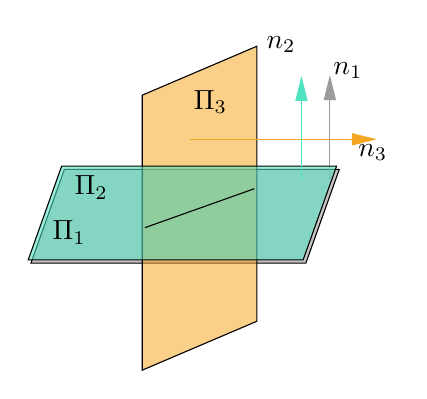
\begin{tikzpicture}[x=0.75pt,y=0.75pt,yscale=-1,xscale=1]
    %uncomment if require: \path (0,310); %set diagram left start at 0, and has height of 310
    
    %Shape: Parallelogram [id:dp6760635656558622] 
    \draw  [fill={rgb, 255:red, 155; green, 155; blue, 155 }  ,fill opacity=0.57 ] (100.2,134.51) -- (232.65,134.51) -- (216.55,179.67) -- (84.09,179.67) -- cycle ;
    %Shape: Parallelogram [id:dp27598068133902265] 
    \draw  [fill={rgb, 255:red, 245; green, 166; blue, 35 }  ,fill opacity=0.54 ] (192.97,75.15) -- (192.97,207.65) -- (137.7,231.24) -- (137.7,98.74) -- cycle ;
    %Straight Lines [id:da42155361486745946] 
    \draw [color={rgb, 255:red, 155; green, 155; blue, 155 }  ,draw opacity=1 ][fill={rgb, 255:red, 155; green, 155; blue, 155 }  ,fill opacity=1 ]   (228.13,139.1) -- (228.13,91.1) ;
    \draw [shift={(228.13,89.1)}, rotate = 90] [fill={rgb, 255:red, 155; green, 155; blue, 155 }  ,fill opacity=1 ][line width=0.08]  [draw opacity=0] (12,-3) -- (0,0) -- (12,3) -- cycle    ;
    %Straight Lines [id:da29239814336841596] 
    \draw [color={rgb, 255:red, 245; green, 166; blue, 35 }  ,draw opacity=1 ][fill={rgb, 255:red, 155; green, 155; blue, 155 }  ,fill opacity=1 ]   (160.66,120) -- (248.7,120) ;
    \draw [shift={(250.7,120)}, rotate = 180] [fill={rgb, 255:red, 245; green, 166; blue, 35 }  ,fill opacity=1 ][line width=0.08]  [draw opacity=0] (12,-3) -- (0,0) -- (12,3) -- cycle    ;
    %Shape: Parallelogram [id:dp8867596814854932] 
    \draw  [fill={rgb, 255:red, 80; green, 227; blue, 194 }  ,fill opacity=0.56 ] (98.9,132.91) -- (231.35,132.91) -- (215.25,178.07) -- (82.79,178.07) -- cycle ;
    %Straight Lines [id:da16327725735587206] 
    \draw [color={rgb, 255:red, 80; green, 227; blue, 194 }  ,draw opacity=1 ][fill={rgb, 255:red, 155; green, 155; blue, 155 }  ,fill opacity=1 ]   (214.43,139.5) -- (214.43,91.5) ;
    \draw [shift={(214.43,89.5)}, rotate = 90] [fill={rgb, 255:red, 80; green, 227; blue, 194 }  ,fill opacity=1 ][line width=0.08]  [draw opacity=0] (12,-3) -- (0,0) -- (12,3) -- cycle    ;
    %Straight Lines [id:da6075265305223774] 
    \draw    (191.74,143.8) -- (138.94,162.6) ;
    
    % Text Node
    \draw (106.27,164.95) node   [align=left] {\begin{minipage}[lt]{17.57pt}\setlength\topsep{0pt}
    $\displaystyle \Pi _{1}$
    \end{minipage}};
    % Text Node
    \draw (174.34,101.88) node   [align=left] {\begin{minipage}[lt]{17.57pt}\setlength\topsep{0pt}
    $\displaystyle \Pi _{3}$
    \end{minipage}};
    % Text Node
    \draw (116.87,143.25) node   [align=left] {\begin{minipage}[lt]{17.57pt}\setlength\topsep{0pt}
    $\displaystyle \Pi _{2}$
    \end{minipage}};
    % Text Node
    \draw (237.47,87.02) node   [align=left] {\begin{minipage}[lt]{11.42pt}\setlength\topsep{0pt}
    $\displaystyle \boldsymbol{n}_{1}$
    \end{minipage}};
    % Text Node
    \draw (205.23,74.53) node   [align=left] {\begin{minipage}[lt]{11.42pt}\setlength\topsep{0pt}
    $\displaystyle \boldsymbol{n}_{2}$
    \end{minipage}};
    % Text Node
    \draw (249.47,126.52) node   [align=left] {\begin{minipage}[lt]{11.42pt}\setlength\topsep{0pt}
    $\displaystyle \boldsymbol{n}_{3}$
    \end{minipage}};
    
    
    \end{tikzpicture}
    
    }
    \subfigure[scale=.9][$r(\vb{A})=r\qty(\bar{\vb{A}})=1$ 有无穷解]{
        

\tikzset{every picture/.style={line width=0.75pt}} %set default line width to 0.75pt        

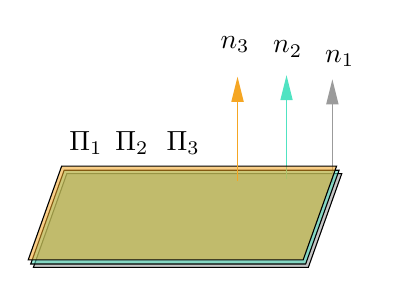
\begin{tikzpicture}[x=0.75pt,y=0.75pt,yscale=-1,xscale=1]
%uncomment if require: \path (0,310); %set diagram left start at 0, and has height of 310

%Shape: Parallelogram [id:dp760070244414208] 
\draw  [fill={rgb, 255:red, 155; green, 155; blue, 155 }  ,fill opacity=0.57 ] (100.2,134.51) -- (232.65,134.51) -- (216.55,179.67) -- (84.09,179.67) -- cycle ;
%Straight Lines [id:da186018516964634] 
\draw [color={rgb, 255:red, 155; green, 155; blue, 155 }  ,draw opacity=1 ][fill={rgb, 255:red, 155; green, 155; blue, 155 }  ,fill opacity=1 ]   (228.13,139.1) -- (228.13,91.1) ;
\draw [shift={(228.13,89.1)}, rotate = 90] [fill={rgb, 255:red, 155; green, 155; blue, 155 }  ,fill opacity=1 ][line width=0.08]  [draw opacity=0] (12,-3) -- (0,0) -- (12,3) -- cycle    ;
%Shape: Parallelogram [id:dp7343355830187419] 
\draw  [fill={rgb, 255:red, 80; green, 227; blue, 194 }  ,fill opacity=0.56 ] (98.9,132.91) -- (231.35,132.91) -- (215.25,178.07) -- (82.79,178.07) -- cycle ;
%Straight Lines [id:da5378006690271788] 
\draw [color={rgb, 255:red, 80; green, 227; blue, 194 }  ,draw opacity=1 ][fill={rgb, 255:red, 155; green, 155; blue, 155 }  ,fill opacity=1 ]   (206.03,137.1) -- (206.03,89.1) ;
\draw [shift={(206.03,87.1)}, rotate = 90] [fill={rgb, 255:red, 80; green, 227; blue, 194 }  ,fill opacity=1 ][line width=0.08]  [draw opacity=0] (12,-3) -- (0,0) -- (12,3) -- cycle    ;
%Shape: Parallelogram [id:dp49950005248676077] 
\draw  [fill={rgb, 255:red, 245; green, 166; blue, 35 }  ,fill opacity=0.54 ] (97.7,130.91) -- (230.15,130.91) -- (214.05,176.07) -- (81.59,176.07) -- cycle ;
%Straight Lines [id:da6548358233391218] 
\draw [color={rgb, 255:red, 245; green, 166; blue, 35 }  ,draw opacity=1 ][fill={rgb, 255:red, 155; green, 155; blue, 155 }  ,fill opacity=1 ]   (182.43,137.9) -- (182.43,89.9) ;
\draw [shift={(182.43,87.9)}, rotate = 90] [fill={rgb, 255:red, 245; green, 166; blue, 35 }  ,fill opacity=1 ][line width=0.08]  [draw opacity=0] (12,-3) -- (0,0) -- (12,3) -- cycle    ;

% Text Node
\draw (113.12,119.73) node   [align=left] {\begin{minipage}[lt]{17.57pt}\setlength\topsep{0pt}
$\displaystyle \Pi _{1}$
\end{minipage}};
% Text Node
\draw (159.94,119.88) node   [align=left] {\begin{minipage}[lt]{17.57pt}\setlength\topsep{0pt}
$\displaystyle \Pi _{3}$
\end{minipage}};
% Text Node
\draw (135.27,119.65) node   [align=left] {\begin{minipage}[lt]{17.57pt}\setlength\topsep{0pt}
$\displaystyle \Pi _{2}$
\end{minipage}};
% Text Node
\draw (232.27,79.02) node   [align=left] {\begin{minipage}[lt]{11.42pt}\setlength\topsep{0pt}
$\displaystyle \boldsymbol{n}_{1}$
\end{minipage}};
% Text Node
\draw (207.23,74.53) node   [align=left] {\begin{minipage}[lt]{11.42pt}\setlength\topsep{0pt}
$\displaystyle \boldsymbol{n}_{2}$
\end{minipage}};
% Text Node
\draw (181.87,72.52) node   [align=left] {\begin{minipage}[lt]{11.42pt}\setlength\topsep{0pt}
$\displaystyle \boldsymbol{n}_{3}$
\end{minipage}};


\end{tikzpicture}

    }
    \subfigure[scale=.9][$r(\vb{A})=2\neq r\qty(\bar{\vb{A}})=3$ 无解]{
        

\tikzset{every picture/.style={line width=0.75pt}} %set default line width to 0.75pt        

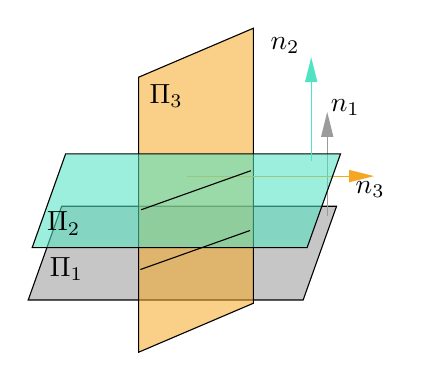
\begin{tikzpicture}[x=0.75pt,y=0.75pt,yscale=-1,xscale=1]
%uncomment if require: \path (0,310); %set diagram left start at 0, and has height of 310

%Shape: Parallelogram [id:dp23267204350760706] 
\draw  [fill={rgb, 255:red, 155; green, 155; blue, 155 }  ,fill opacity=0.57 ] (100.2,134.51) -- (232.65,134.51) -- (216.55,179.67) -- (84.09,179.67) -- cycle ;
%Shape: Parallelogram [id:dp028553730591406534] 
\draw  [fill={rgb, 255:red, 245; green, 166; blue, 35 }  ,fill opacity=0.54 ] (192.57,48.75) -- (192.57,181.25) -- (137.3,204.84) -- (137.3,72.34) -- cycle ;
%Straight Lines [id:da42377076903338984] 
\draw [color={rgb, 255:red, 155; green, 155; blue, 155 }  ,draw opacity=1 ][fill={rgb, 255:red, 155; green, 155; blue, 155 }  ,fill opacity=1 ]   (228.13,139.1) -- (228.13,91.1) ;
\draw [shift={(228.13,89.1)}, rotate = 90] [fill={rgb, 255:red, 155; green, 155; blue, 155 }  ,fill opacity=1 ][line width=0.08]  [draw opacity=0] (12,-3) -- (0,0) -- (12,3) -- cycle    ;
%Straight Lines [id:da5299339204120483] 
\draw [color={rgb, 255:red, 245; green, 166; blue, 35 }  ,draw opacity=1 ][fill={rgb, 255:red, 155; green, 155; blue, 155 }  ,fill opacity=1 ]   (160.66,120) -- (248.7,120) ;
\draw [shift={(250.7,120)}, rotate = 180] [fill={rgb, 255:red, 245; green, 166; blue, 35 }  ,fill opacity=1 ][line width=0.08]  [draw opacity=0] (12,-3) -- (0,0) -- (12,3) -- cycle    ;
%Shape: Parallelogram [id:dp7848313018899085] 
\draw  [fill={rgb, 255:red, 80; green, 227; blue, 194 }  ,fill opacity=0.56 ] (102.1,109.31) -- (234.55,109.31) -- (218.45,154.47) -- (85.99,154.47) -- cycle ;
%Straight Lines [id:da6086045301320668] 
\draw [color={rgb, 255:red, 80; green, 227; blue, 194 }  ,draw opacity=1 ][fill={rgb, 255:red, 155; green, 155; blue, 155 }  ,fill opacity=1 ]   (220.43,112.7) -- (220.43,64.7) ;
\draw [shift={(220.43,62.7)}, rotate = 90] [fill={rgb, 255:red, 80; green, 227; blue, 194 }  ,fill opacity=1 ][line width=0.08]  [draw opacity=0] (12,-3) -- (0,0) -- (12,3) -- cycle    ;
%Straight Lines [id:da012761391879912543] 
\draw    (190.94,146.2) -- (138.14,165) ;
%Straight Lines [id:da3251143183119318] 
\draw    (191.34,117.4) -- (138.54,136.2) ;

% Text Node
\draw (106.27,164.95) node   [align=left] {\begin{minipage}[lt]{17.57pt}\setlength\topsep{0pt}
$\displaystyle \Pi _{1}$
\end{minipage}};
% Text Node
\draw (154.34,81.48) node   [align=left] {\begin{minipage}[lt]{17.57pt}\setlength\topsep{0pt}
$\displaystyle \Pi _{3}$
\end{minipage}};
% Text Node
\draw (104.87,142.85) node   [align=left] {\begin{minipage}[lt]{17.57pt}\setlength\topsep{0pt}
$\displaystyle \Pi _{2}$
\end{minipage}};
% Text Node
\draw (237.47,87.02) node   [align=left] {\begin{minipage}[lt]{11.42pt}\setlength\topsep{0pt}
$\displaystyle \boldsymbol{n}_{1}$
\end{minipage}};
% Text Node
\draw (208.43,56.93) node   [align=left] {\begin{minipage}[lt]{11.42pt}\setlength\topsep{0pt}
$\displaystyle \boldsymbol{n}_{2}$
\end{minipage}};
% Text Node
\draw (249.47,126.52) node   [align=left] {\begin{minipage}[lt]{11.42pt}\setlength\topsep{0pt}
$\displaystyle \boldsymbol{n}_{3}$
\end{minipage}};


\end{tikzpicture}

    }
    \subfigure[scale=.9][$r(\vb{A})=2\neq r\qty(\bar{\vb{A}})=3$ 无解]{
        

\tikzset{every picture/.style={line width=0.75pt}} %set default line width to 0.75pt        

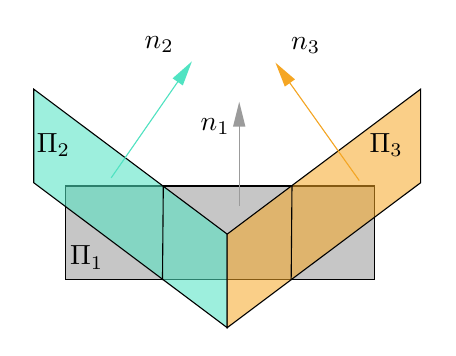
\begin{tikzpicture}[x=0.75pt,y=0.75pt,yscale=-1,xscale=1]
%uncomment if require: \path (0,310); %set diagram left start at 0, and has height of 310

%Shape: Parallelogram [id:dp237593131096703] 
\draw  [fill={rgb, 255:red, 155; green, 155; blue, 155 }  ,fill opacity=0.57 ] (103.59,128.01) -- (252.15,128.01) -- (252.15,173.17) -- (103.59,173.17) -- cycle ;
%Shape: Parallelogram [id:dp30557238360563566] 
\draw  [fill={rgb, 255:red, 80; green, 227; blue, 194 }  ,fill opacity=0.56 ] (181.34,151.17) -- (181.34,196.24) -- (88.14,126.41) -- (88.14,81.33) -- cycle ;
%Shape: Parallelogram [id:dp8537926266308529] 
\draw  [fill={rgb, 255:red, 245; green, 166; blue, 35 }  ,fill opacity=0.54 ] (274.53,81.33) -- (274.53,126.41) -- (181.34,196.24) -- (181.34,151.17) -- cycle ;
%Straight Lines [id:da03271360553568958] 
\draw [color={rgb, 255:red, 155; green, 155; blue, 155 }  ,draw opacity=1 ][fill={rgb, 255:red, 155; green, 155; blue, 155 }  ,fill opacity=1 ]   (187.13,137.4) -- (187.13,89.4) ;
\draw [shift={(187.13,87.4)}, rotate = 90] [fill={rgb, 255:red, 155; green, 155; blue, 155 }  ,fill opacity=1 ][line width=0.08]  [draw opacity=0] (12,-3) -- (0,0) -- (12,3) -- cycle    ;
%Straight Lines [id:da8824637174339032] 
\draw [color={rgb, 255:red, 245; green, 166; blue, 35 }  ,draw opacity=1 ][fill={rgb, 255:red, 155; green, 155; blue, 155 }  ,fill opacity=1 ]   (244.96,125.36) -- (205.76,70.2) ;
\draw [shift={(204.6,68.57)}, rotate = 54.6] [fill={rgb, 255:red, 245; green, 166; blue, 35 }  ,fill opacity=1 ][line width=0.08]  [draw opacity=0] (12,-3) -- (0,0) -- (12,3) -- cycle    ;
%Straight Lines [id:da627926502859631] 
\draw [color={rgb, 255:red, 80; green, 227; blue, 194 }  ,draw opacity=1 ][fill={rgb, 255:red, 155; green, 155; blue, 155 }  ,fill opacity=1 ]   (125.43,124.09) -- (163.19,69.61) ;
\draw [shift={(164.33,67.97)}, rotate = 124.73] [fill={rgb, 255:red, 80; green, 227; blue, 194 }  ,fill opacity=1 ][line width=0.08]  [draw opacity=0] (12,-3) -- (0,0) -- (12,3) -- cycle    ;
%Straight Lines [id:da07462088125718092] 
\draw    (150.56,127.76) -- (150.16,173.36) ;
%Straight Lines [id:da9124947874861398] 
\draw    (212.56,127.76) -- (212.16,173.36) ;

% Text Node
\draw (117.37,162.45) node   [align=left] {\begin{minipage}[lt]{17.57pt}\setlength\topsep{0pt}
$\displaystyle \Pi _{1}$
\end{minipage}};
% Text Node
\draw (261.64,108.18) node   [align=left] {\begin{minipage}[lt]{17.57pt}\setlength\topsep{0pt}
$\displaystyle \Pi _{3}$
\end{minipage}};
% Text Node
\draw (101.37,108.45) node   [align=left] {\begin{minipage}[lt]{17.57pt}\setlength\topsep{0pt}
$\displaystyle \Pi _{2}$
\end{minipage}};
% Text Node
\draw (176.17,99.22) node   [align=left] {\begin{minipage}[lt]{11.42pt}\setlength\topsep{0pt}
$\displaystyle \boldsymbol{n}_{1}$
\end{minipage}};
% Text Node
\draw (149.23,60.02) node   [align=left] {\begin{minipage}[lt]{11.42pt}\setlength\topsep{0pt}
$\displaystyle \boldsymbol{n}_{2}$
\end{minipage}};
% Text Node
\draw (219.77,60.42) node   [align=left] {\begin{minipage}[lt]{11.42pt}\setlength\topsep{0pt}
$\displaystyle \boldsymbol{n}_{3}$
\end{minipage}};


\end{tikzpicture}

    }
    \subfigure[scale=.9][$r(\vb{A})=1\neq r\qty(\bar{\vb{A}})=2$ 无解]{
        

\tikzset{every picture/.style={line width=0.75pt}} %set default line width to 0.75pt        

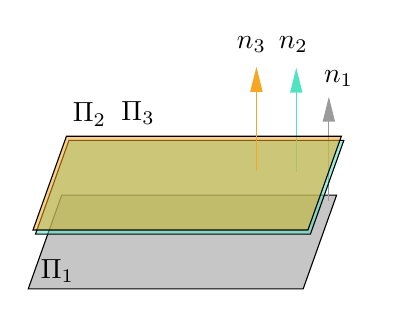
\begin{tikzpicture}[x=0.75pt,y=0.75pt,yscale=-1,xscale=1]
%uncomment if require: \path (0,310); %set diagram left start at 0, and has height of 310

%Shape: Parallelogram [id:dp4962533776252094] 
\draw  [fill={rgb, 255:red, 155; green, 155; blue, 155 }  ,fill opacity=0.57 ] (101.8,117.71) -- (234.25,117.71) -- (218.15,162.87) -- (85.69,162.87) -- cycle ;
%Straight Lines [id:da890876705178447] 
\draw [color={rgb, 255:red, 155; green, 155; blue, 155 }  ,draw opacity=1 ][fill={rgb, 255:red, 155; green, 155; blue, 155 }  ,fill opacity=1 ]   (230.53,120.3) -- (230.53,72.3) ;
\draw [shift={(230.53,70.3)}, rotate = 90] [fill={rgb, 255:red, 155; green, 155; blue, 155 }  ,fill opacity=1 ][line width=0.08]  [draw opacity=0] (12,-3) -- (0,0) -- (12,3) -- cycle    ;
%Shape: Parallelogram [id:dp3332922227144113] 
\draw  [fill={rgb, 255:red, 80; green, 227; blue, 194 }  ,fill opacity=0.56 ] (105.3,91.31) -- (237.75,91.31) -- (221.65,136.47) -- (89.19,136.47) -- cycle ;
%Straight Lines [id:da44458743956600877] 
\draw [color={rgb, 255:red, 80; green, 227; blue, 194 }  ,draw opacity=1 ][fill={rgb, 255:red, 155; green, 155; blue, 155 }  ,fill opacity=1 ]   (214.83,106.3) -- (214.83,58.3) ;
\draw [shift={(214.83,56.3)}, rotate = 90] [fill={rgb, 255:red, 80; green, 227; blue, 194 }  ,fill opacity=1 ][line width=0.08]  [draw opacity=0] (12,-3) -- (0,0) -- (12,3) -- cycle    ;
%Shape: Parallelogram [id:dp8959701963986486] 
\draw  [fill={rgb, 255:red, 245; green, 166; blue, 35 }  ,fill opacity=0.54 ] (104.1,89.31) -- (236.55,89.31) -- (220.45,134.47) -- (87.99,134.47) -- cycle ;
%Straight Lines [id:da17960473590380155] 
\draw [color={rgb, 255:red, 245; green, 166; blue, 35 }  ,draw opacity=1 ][fill={rgb, 255:red, 155; green, 155; blue, 155 }  ,fill opacity=1 ]   (195.63,105.9) -- (195.63,57.9) ;
\draw [shift={(195.63,55.9)}, rotate = 90] [fill={rgb, 255:red, 245; green, 166; blue, 35 }  ,fill opacity=1 ][line width=0.08]  [draw opacity=0] (12,-3) -- (0,0) -- (12,3) -- cycle    ;

% Text Node
\draw (103.52,154.13) node   [align=left] {\begin{minipage}[lt]{17.57pt}\setlength\topsep{0pt}
$\displaystyle \Pi _{1}$
\end{minipage}};
% Text Node
\draw (142.34,78.28) node   [align=left] {\begin{minipage}[lt]{17.57pt}\setlength\topsep{0pt}
$\displaystyle \Pi _{3}$
\end{minipage}};
% Text Node
\draw (118.87,78.85) node   [align=left] {\begin{minipage}[lt]{17.57pt}\setlength\topsep{0pt}
$\displaystyle \Pi _{2}$
\end{minipage}};
% Text Node
\draw (235.87,61.42) node   [align=left] {\begin{minipage}[lt]{11.42pt}\setlength\topsep{0pt}
$\displaystyle \boldsymbol{n}_{1}$
\end{minipage}};
% Text Node
\draw (214.03,45.33) node   [align=left] {\begin{minipage}[lt]{11.42pt}\setlength\topsep{0pt}
$\displaystyle \boldsymbol{n}_{2}$
\end{minipage}};
% Text Node
\draw (193.87,45.32) node   [align=left] {\begin{minipage}[lt]{11.42pt}\setlength\topsep{0pt}
$\displaystyle \boldsymbol{n}_{3}$
\end{minipage}};


\end{tikzpicture}

    }
    \subfigure[scale=.9][$r(\vb{A})=1\neq r\qty(\bar{\vb{A}})=3$ 无解]{
        

\tikzset{every picture/.style={line width=0.75pt}} %set default line width to 0.75pt        

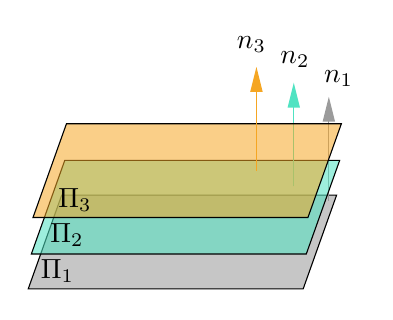
\begin{tikzpicture}[x=0.75pt,y=0.75pt,yscale=-1,xscale=1]
%uncomment if require: \path (0,310); %set diagram left start at 0, and has height of 310

%Shape: Parallelogram [id:dp4962533776252094] 
\draw  [fill={rgb, 255:red, 155; green, 155; blue, 155 }  ,fill opacity=0.57 ] (101.8,117.71) -- (234.25,117.71) -- (218.15,162.87) -- (85.69,162.87) -- cycle ;
%Straight Lines [id:da890876705178447] 
\draw [color={rgb, 255:red, 155; green, 155; blue, 155 }  ,draw opacity=1 ][fill={rgb, 255:red, 155; green, 155; blue, 155 }  ,fill opacity=1 ]   (230.53,120.3) -- (230.53,72.3) ;
\draw [shift={(230.53,70.3)}, rotate = 90] [fill={rgb, 255:red, 155; green, 155; blue, 155 }  ,fill opacity=1 ][line width=0.08]  [draw opacity=0] (12,-3) -- (0,0) -- (12,3) -- cycle    ;
%Shape: Parallelogram [id:dp3332922227144113] 
\draw  [fill={rgb, 255:red, 80; green, 227; blue, 194 }  ,fill opacity=0.56 ] (103.3,100.91) -- (235.75,100.91) -- (219.65,146.07) -- (87.19,146.07) -- cycle ;
%Straight Lines [id:da44458743956600877] 
\draw [color={rgb, 255:red, 80; green, 227; blue, 194 }  ,draw opacity=1 ][fill={rgb, 255:red, 155; green, 155; blue, 155 }  ,fill opacity=1 ]   (213.63,113.5) -- (213.63,65.5) ;
\draw [shift={(213.63,63.5)}, rotate = 90] [fill={rgb, 255:red, 80; green, 227; blue, 194 }  ,fill opacity=1 ][line width=0.08]  [draw opacity=0] (12,-3) -- (0,0) -- (12,3) -- cycle    ;
%Shape: Parallelogram [id:dp8959701963986486] 
\draw  [fill={rgb, 255:red, 245; green, 166; blue, 35 }  ,fill opacity=0.54 ] (104.1,83.31) -- (236.55,83.31) -- (220.45,128.47) -- (87.99,128.47) -- cycle ;
%Straight Lines [id:da17960473590380155] 
\draw [color={rgb, 255:red, 245; green, 166; blue, 35 }  ,draw opacity=1 ][fill={rgb, 255:red, 155; green, 155; blue, 155 }  ,fill opacity=1 ]   (195.63,105.9) -- (195.63,57.9) ;
\draw [shift={(195.63,55.9)}, rotate = 90] [fill={rgb, 255:red, 245; green, 166; blue, 35 }  ,fill opacity=1 ][line width=0.08]  [draw opacity=0] (12,-3) -- (0,0) -- (12,3) -- cycle    ;

% Text Node
\draw (103.52,154.13) node   [align=left] {\begin{minipage}[lt]{17.57pt}\setlength\topsep{0pt}
$\displaystyle \Pi _{1}$
\end{minipage}};
% Text Node
\draw (111.94,119.88) node   [align=left] {\begin{minipage}[lt]{17.57pt}\setlength\topsep{0pt}
$\displaystyle \Pi _{3}$
\end{minipage}};
% Text Node
\draw (108.07,136.85) node   [align=left] {\begin{minipage}[lt]{17.57pt}\setlength\topsep{0pt}
$\displaystyle \Pi _{2}$
\end{minipage}};
% Text Node
\draw (235.87,61.42) node   [align=left] {\begin{minipage}[lt]{11.42pt}\setlength\topsep{0pt}
$\displaystyle \boldsymbol{n}_{1}$
\end{minipage}};
% Text Node
\draw (214.83,52.53) node   [align=left] {\begin{minipage}[lt]{11.42pt}\setlength\topsep{0pt}
$\displaystyle \boldsymbol{n}_{2}$
\end{minipage}};
% Text Node
\draw (193.87,45.32) node   [align=left] {\begin{minipage}[lt]{11.42pt}\setlength\topsep{0pt}
$\displaystyle \boldsymbol{n}_{3}$
\end{minipage}};


\end{tikzpicture}

    }
    \caption{}
    \label{mianmiangx}
\end{figure}

\subsection{无解方程组的最小误差解}

\begin{theorem}[最小二乘解]
    方程组 $\vb*{Ax}=\vb*{b}$ 的最小二乘解为 $\vb*{x}=\qty(\vb*{A}^\top\vb*{A})^{-1}\vb*{A}^\top\vb*{b}$.
    \index{最小二乘解}
\end{theorem}